\documentclass[fourier]{_style/dissertation}
\usepackage{hyperref}
\usepackage{algorithm}
\usepackage{algpseudocode}
\usepackage{listings}
\lstdefinestyle{mystyle}{
    backgroundcolor=\color{backcolour},   
    commentstyle=\color{codegreen},
    keywordstyle=\color{magenta},
    numberstyle=\tiny\color{codegray},
    stringstyle=\color{codepurple},
    basicstyle=\ttfamily\footnotesize,
    breakatwhitespace=false,         
    breaklines=true,                 
    captionpos=b,                    
    keepspaces=true,                 
    numbers=left,                    
    numbersep=5pt,                  
    showspaces=false,                
    showstringspaces=false,
    showtabs=false,                  
    tabsize=2
}
\lstset{style=mystyle}
\hyphenation{ge-for-der-te sus-pen-dier-ten}

\addbibresource[glob]{*.bib}
\title[Learn personalized model that predicts \textbf{EMG} Signals while Keeping user's privacy]{Personalized Differentialy Private Federated Learning}
\author{Moshe}{Beutel}

\begin{document}
\begin{titlepage}
    \begin{center}
        \vspace*{2\bigskipamount}
        {\makeatletter
            \titlestyle\bfseries\LARGE Bar-Ilan University \\
            The Faculty of Engineering \\
            \bigskip
            Electrical Engineering, Data Science Track \\
            \bigskip
            MSc. Research Proposal
            \makeatother}
        \bigskip
        \bigskip
        \bigskip

    \end{center} 
      \textbf{Research Subject:} 
     \begin{center}
         
        
        \bigskip
        {\makeatletter
            \titlestyle\bfseries\LARGE 
            \@title
            \makeatother}

        %% Print the optional subtitle.
        {\makeatletter
            \ifx\@subtitle\undefined\else
                \bigskip
                \titlefont\titleshape\Large\@subtitle
            \fi
            \makeatother}
        \vfill
        \makeatletter
        \begin{tabular}{ c c }
             Student: &   {\Large\titlefont\bfseries\@firstnames\ {\Large\titlefont\bfseries\@lastname}}  \\ 
             Supervisor:  & {\Large\titlefont\bfseries Dr. Ethan  {\Large\titlefont\bfseries Fetaya}}    
        \end{tabular}
        
        \makeatother
        \vspace*{2\bigskipamount}

    \end{center}
\end{titlepage}

{
  % \cleardoublepage%
  \phantomsection%
  \pdfbookmark[1]{\contentsname}{toc}
  \tableofcontents
}

\chapter{Introduction}
\section{EMG}
The rapid growth of wearable technology and the increasing availability of electromyography (\textbf{EMG}) wrist devices have opened up new possibilities for monitoring and analyzing human movements. \\

\subsection{The putEMG Dataset}
The putEMG dataset \cite{Kaczmarek2019PutEMGADataset} contains multi-channel surface electromyographic activity recorded from forearm. 
\subsubsection{Experiment Procedures}
Experiments were originally conducted on 44 participants. At each session the participant wore a 24 (8x3) electrode matrix and performed a series of 7 different actions separated by an idle state:
\begin{itemize}
    \item 0 - Idle state
    \item 1 - Fist
    \item 2 - Flexion
    \item 3 - Extension
    \item 6 - Pinch index
    \item 7 - Pinch middle
    \item 8 - Pinch ring
    \item 9 - Pinch small
\end{itemize}

\textit{Action Block} - The basic experiment procedure. A series of gestures and idle states performed as follows:\\

\textbf{for} $i$ in \textit{action\_set}:
\begin{enumerate}
    \item  \textbf{Do} gesture $i$ for $1$ or $3$ seconds (depending on trajectory - more on this later)
    \item   \textbf{Do} idle gesture for $3$ seconds
\end{enumerate}
 Between action blocks user were able to relax and move their hands freely for 10 seconds. A relax period is marked as -1. Each action block begins and ends with an idle gesture.

\textit{Trajectory} - A series of action blocks separated by relax periods.\\
Trajectory Types - 
\begin{itemize}
    \item \textit{repeats\_long} - 7 action blocks, each block contains 8 repetitions of each active gesture: [relax] 0-1-0-1-0-1-0-1-0-1-0-1-0-1-0-1-0 [relax] 0-2-0-2-0-2-0-2-0-2-0-2-0-2-0-2-0 [relax] 0-3-0... ,
    \item \textit{sequential} - 6 action blocks, each block is a subsequent execution of all active gestures: [relax] 0-1-0-2-0-3-0-6-0-7-0-8-0-9-0 [relax] 0-1-0-2-0-3-0-6-0-7-0-8-0-9-0 [relax] 0-1-0-2-0... ,
    \item \textit{repeats\_short} - 7 action blocks, each block contains 6 repetitions of each active gesture: [relax] 0-1-0-1-0-1-0-1-0-1-0-1-0 [relax] 0-2-0-2-0-2-0-2-0-2-0-2-0 [relax] 0-3-0... .
\end{itemize}
In a single experiment session a user performed the 3 trajectory types once which is summed to repeat each gesture 20 times.

Each participant had 2 sessions separated by minimum one week.

\subsection{Dataset Structure}
The dataset contains a csv file per user experiments (44 users X 2 Experiment sessions X 3 trajectory types = 264 files).
Each csv file contains a data frame with the following columns:
\begin{itemize}
    \item 24 EMG\_$i$ columns (1 per electrode) - The raw ADC signal value. A raw ADC signal read can be converted to milivolot using the following formula:
    $$N \rightarrow \frac{N \cdot 5}{2^{12}}\frac{1000}{200}[mV]$$
    \item TRAJ\_1- The gesture that was presented to the participant
    \item TRAJ\_GT\_NO\_FILTER - Gesture labeling using video stream gesture recognition algorithm. A VGGNet based recognition with no filter.
    \item TRAJ\_GT - The output of the median filter applied to the VGGNet and a window of 250 ms before presenting the action $i$ to 2000 ms after presenting the next action where outside this window action $i$ was discarded. \\ \textit{This column values were taken as ground true for the purpose of this research.}
    
\end{itemize}

\section{The Privacy Problem}

The EMG data collected from wrist devices contains personal information about users' hand movements, gestures, and muscle activity. This sensitive data could be exploited by malicious hackers with the intent to harm users or steal their identity. \\

Moreover, the increasing adoption of EMG data in various applications, such as rehabilitation, virtual reality, and human-computer interaction, highlights the need for accurate models. Accurate models need a large amount of data to be learned \\

EMG data must be safeguarded for privacy reasons, whereas EMG models require a substantial amount of data for effective training. These two objectives are not inherently aligned. \\



The objective of this thesis proposal is to learn a machine learning model of EMG data in a federated manner such that differential privacy is kept and accuracy is as good as we can get. By preserving the privacy of individual users while enabling robust analysis, we aim to strike a balance between privacy preservation and data utility. Additionally, we propose a novel approach that involves leveraging public users to embed gradients onto their subspace, further enhancing the privacy guarantees.\\

\section{Weak Privacy and Strong Privacy}
Learning a gesture classifier in a \textbf{Federated} manner makes use of large population data while not pulling personal sensitive data from the wearable device. Moreover, federated learning has the advantage of personalizing model inference to a specific user. \\

But as demonstrated in the Netflix Prize competition, a renowned competition in the field of recommendation systems, \textbf{data anonymization does not ensure privacy}. While the contest aimed to improve movie recommendations by encouraging data sharing and algorithm development, it inadvertently exposed the potential risks of de-anonymization when researchers were able to de-anonymize users' personal data by cross referencing models trained on Netflix anonymized data with the IMDb dataset which is not anonymized. This event demonstrated how seemingly anonymized data can be de-anonymized when combined with additional information. 

A proposed technique to address this concern is \textbf{Differential privacy} \cite{Dwork2013ThePrivacy}. \\
Differential privacy offers a rigorous framework for privacy preservation in data analysis while still allowing valuable insights to be derived from the data. By introducing carefully calibrated noise into the computation process, it ensures that individual data points - in our case individual users -  remain indistinguishable in the final analysis results. This statistical privacy concept provides a formal and provable guarantee of privacy, even when an adversary has access to auxiliary information.\\

The \textbf{DP-SGD} \cite{Abadi2016DeepPrivacy} method is an efficient way to incorporate differential privacy to deep learning model. DP-SGD adds noise to the gradients before gradients are backpropagetd through the network. Moreover, DP-SGD computes the amount of privacy spent at each learning step and at the overall learning process. 

The \textbf{GEP} \cite{Yu2021DoLearning} proposes a method for estimating model gradients during training by incorporating them into a lower-rank subspace. Subsequently, privacy noise is introduced to the incorporated gradients. The motivation is that less noise is needed for the same amount of privacy. \\

\section{Our Contribution - Performance of Differential Private Federated Learning U sing Public Users }
Although effective, DP-SGD and GEP still exhibit a reduction in performance. To enhance the performance of EMG data models inference while maintaining privacy assurances, we propose a novel approach that relies on the participation of \textbf{public users} who are willing to expose their data. The public users' data is used for gradient subspace computation that all private gradients will be embedded into. We assume that the more gradients' "energy" is concentrated in the embedding subspace, the learned model will perform better.\\

\section{Federated Learning}
In the \textit{Federated Learning} (\textbf{FL}) setup multiple clients collaborate to solve a machine learning problem under some central aggregator. This setup is increasingly attractive with the rise of mobile smartphones wearable devices, IoT and smart homes. FL rises a few theoretical and technical challenges.

\subsection{Federated Learning Formal Definition}
\textbf{Definition}: $N$ users, $\{U_{1},...,U_{n}\}$ each of them owns a database  $\{D_{1},...,D_{n} \}$ respectively, where $U_{i}$ can access $D_{j}$ iff $i=j$. I federated learning learns a model by collecting training information from the different users. Usually this is done in the following schema.
\begin{itemize}
    \item Server sends initial model $\theta_{0}$ to clients.
    \item $U_{i}$ trains the model using $D_{i}$.
    \item Server aggregates local models $\theta_{0,i}$ to construct a global model.
    \item Server sends updated model $\theta_{1}$ to clients.
\end{itemize}
The above schema can of course be repeated multiple times till convergence.

\subsection{FL Challenges}
\begin{itemize}
    \item \textbf{Massively Distributed} - $\# \{ \text{Clients} \} > >  \# \{ \text{Data per Client} \}$
    \item \textbf{Non-IID} - The data distribution at specific client does not represent the global population.
    \item \textbf{Unbalanced} - Users produce significantly different amount of data due to device use habits.
    \item \textbf{Limited Communication} - Some clients may be offline frequently or have limited connectivity. Therefore, not available for sampling or model updates.               
    \item \textbf{User Privacy} - Although data is not pulled out of user device privacy is not guaranteed and differential privacy methods should be applied.
    \item \textbf{Personalization} - Tailoring a machine learning model to an individual user's preferences, needs, or characteristics by model adaptation at the edge. One such adaptation of the model is inferring by a Gaussian Process that uses the global model as its backbone.
\end{itemize}

\section{Differential Privacy}
The definitions and theorems in this section are taken from \cite{Dwork2014ThePrivacy}. \\
Given $D \sim D'$ datasets that differs at exactly a single entry, A $(\epsilon,\delta)$-DP algorithm $\mathcal{M}$'s outputs difference is bounded such that an adversary cannot infer the difference between $D$ and $D'$ using  $\mathcal{M}$. \\
% M's outcome does not expose the data up to a certain privacy budget controlled by $(\epsilon, \delta)$. \\  
Formally, Given $\epsilon>0, \delta \in [0,1]$ if for every such (D,D')  
$$  Pr[M(D) \in O] \leq e^{\epsilon}Pr[\mathcal{M}(D') \in O]+ \delta$$ for all measurable sets $O \subseteq \texttt{range}(M)$ the randomized algorithm M is called $(\epsilon,\delta)$-DP. \\

The meaning of $(\epsilon, \delta)$ parameters - \\
\begin{itemize}
    \item $\epsilon$ is called the \textit{privacy parameter} or the \textit{privacy budget} and is the amount of privacy we \textbf{know} we loose by $\mathcal{M}$. 
    \item $\delta$ is the probability of \textbf{accidental} leakage.
\end{itemize}


\subsection{Sensitivity}
\textbf{Local Sensitivity} - \\
The \textit{Local Sensitivity} of a function $h:\mathbb{R}^{n}\rightarrow\mathbb{R} \cup \{\infty\}$ is defined as: 
$$LS_{h}(x)=\sup\{\|h(x')-h(x)\|x'\in\mathbb{R}^{n},d_{H}(x,x')\leq 1 \}$$
The maximum change in the output h for changing the dataset $x$ with a dataset that differs at most in a single entry. \\
\textbf{Global Sensitivity} - \\
The Global Sensitivity is the supremum of all Local Sensitivities 
$$GS_{H}=\sup\limits_{x\in\mathbb{R}^{n}}\{LS_{h}(x)\}$$
Since the definition of sensitivity involves norms, it is closely dependant on the underling metric. We define the metric on \textit{Numeric Queries} - functions that map databases to k real numbers -  $f: \mathbb{N}^{|\chi|} \leftarrow \mathbb{R}^{k}$.\\
\textbf{Definition:} The $l_{1}$-sensitivity of a function $f: \mathbb{N}^{|\chi|} \leftarrow \mathbb{R}^{k}$ is: 
$$ \Delta f = \max_{x,y \in \mathbb{N}^{|\chi|}, ||x-y||_{1}=1} || f(x) - f(y) ||_{1}.$$
and similarly \\
\textbf{Definition:} The $l_{2}$-sensitivity of a function $f: \mathbb{N}^{|\chi|} \leftarrow \mathbb{R}^{k}$ is: 
$$ \Delta f = \max_{x,y \in \mathbb{N}^{|\chi|}, ||x-y||_{1}=1} || f(x) - f(y) ||_{2}.$$
In the following section we will see that the $l_{1}$-sensitivity is related to the \textit{Laplace Mechanism} and and the $l_{2}$-sensitivity is related to the \textit{Gaussian Mechanism}.
\subsection{Differential Privacy Mechanisms}
The most common way to achieve differential privacy is adding noise to the algorithm the data processing algorithm or the learning algorithm. Two common noise types are Laplace Noise and Gaussian Noise.
\subsubsection{Laplace Mechanism}
The Laplace Mechanism adds a Laplace distributed noise. \\
\textbf{Definition:} The \textit{Laplace Distribution} with mean 0 and standard deviation $\sqrt{2} \sigma$ has probability density:
$$ Lap(x|\sigma)=\frac{1}{2\sigma}\exp \left (- \frac{|x|}{\sigma} \right ).$$ $\sigma$ is the Laplace distribution parameter and a r.v. $X$ drawn from it is noted $X \sim Lap(\sigma)$.
The Laplace Mechanism is therefore: \\
\textbf{Definition:} Given any function $f:\mathbb{N}^{|\chi|} \leftarrow \mathbb{R}^{k}$, \textit{The Laplace Mechanism} is defined as:
$$ \mathcal{M}_{L}(x,f(\cdot), \epsilon) = f(x)+(Y_{1},\ldots ,Y_{k})$$
where $Y_{i} \sim Lap(\Delta f / \epsilon)$ i.i.d.
The following theorem states that the Laplace Mechanism ensures Differential Privacy to a given budget. \\
\textbf{Theorem:} The Laplace Mechanism preserves $(\epsilon, 0)$-differential privacy.
\subsubsection{Gaussian Mechanism}
The Gaussian Mechanism adds Gaussian noise. \\
\textbf{Definition:} The \textit{Gaussian Mechanism} with 0 mean and parameter $\sigma$ adds Gaussian noise distributed $\sim \mathbf{N}(0,\sigma^{2})$ to each of the output's $k$ dimensions.\\
\textbf{Theorem:} Let $\epsilon \in (0,1)$. For $c^{2} > 2 \ln(1.25/\delta)$, the \textit{Gaussian Mechanism} with parameter $\sigma \geq c\Delta_{2}(f)/\epsilon$ is $(\epsilon, \delta)$-differentialy private.

\subsection{Gradient Embedding Perturbation (GEP)}
\label{GEP}
\cite{Yu2021DoLearning} presents the Gradient Embedding Perturbation (GEP) algorithm. The motivation behind GEP is that the gradients live in some manifold while the noise added to them is isotropic so we wish to first reduce the dimension of the gradients and then add the noise. The main trick of the GEP algorithm is use an \textit{anchor subspace} which is constructed as follows. Using an auxiliary, non-sensitive, dataset $\mathbb{D}^{(a)}$ that contains $m$ samples, compute an anchor gradients $G^{(a)} \in \mathbb{R}^{m \times p}$. Estimate the principal components of the anchor gradients using power methods to construct the subspace basis $B \in \mathbb{R}^{k \times p}$ which is the \textit{anchor subspace}. Since the auxiliary dataset is similar to the private dataset we expect the anchor subspace $B$ to express the private gradients as well. 

GEP algorithm can thus be described as follows: 
\begin{enumerate}
    \item Estimate an anchor subspace that contains the principal components of some non-sensitive anchor gradients via power methods. The anchor subspace is constructed as follows. 
    \item Project the private gradients $G \in \mathbb{R}^{n \times p}$ into the anchor subspace $B$ and produce low-dimensional embedding $W=GB^{T}$ of private gradients and  residual gradients  $R=G-GB^{T}B$ which have much smaller magnitude. Use $S_{1}$ threshold to clip $W$'s rows and obtain $\hat{W}$, and use $S_{2}$ threshold to clip $R$'s rows to obtain $\hat{R}$.
    \item Aggregate the gradient embedding the residual embedding \textbf{separately}  and perturb each of these aggregations with Gaussian noise.
    \begin{itemize}
        \item Embedding aggregation perturbation:  $z^{(1)} \sim \mathbf{N}(0, \sigma_{1}^{2}I_{k \times k}): w:=\sum_{i} \hat{W}_{i}, \Tilde{w}:=w+z^{(1)}$. 
        \item Residual gradients aggregation perturbation: $z^{(2)} \sim \mathbf{N}(0,\sigma_{2}^{2}I_{p \times p}): r:=\sum_{i} \hat{R}_{i}, \Tilde{r}:=r+z^{(2)}$
        \item Unbiased estimator of the private gradient: $\Tilde{v}:=(\Tilde{w}^{T}B+\Tilde{r})/n$
    \end{itemize}
    
    
\end{enumerate}

\section{Gaussian Processes}

\subsection{Gaussian Process Definition}
\textbf{Definition:} A Gaussian Process (GP) \cite{Rasmussen2006Gaussian2006} is a collection of random variables where any finite subset of these variables are jointly Gaussian. \\
One can view a GP as a distribution over functions where a random function $f:R^{n} \rightarrow R^{m}$ sampled from some GP has a mean value defined by a mean function $\mu: R^{n} \rightarrow R^{m}$ and covariance function between different $f$ values defined by a kernel function $k(x,x'): (R^{n}, R^{n}) \rightarrow R^{m} $ 
Formally,
$$f(x) \sim GP(\mu(x), k(x,x')),$$ where $$\mu(x)=E[f(x)]$$ $$k(x,x')=E[(f(x)-\mu(x))(f(x')-\mu(x))]$$ 

There are several families of kernel functions of which the most popular/trivial is called the \textit{Squared Exponential} or \textit{Radial Basis Function} (\textbf{RBF}) which is defined as: \\
$$k(x,x')=\sigma^{2} exp(-\frac{\lVert x-x' \rVert ^{2}}{2l^{2}})$$. The hyperparameters are: \\
\begin{itemize}
    \item $\sigma$ - The prior \textit{standard deviation} - Controls each individual values vary
    \item $l$ - The \textit{lengthscale} - Controls how distant input values affect each other
\end{itemize}

\subsection{Variational Inference and Inducing Points}
GPs have a natural problem with scaling to large datasets. Computation needs $O(n^{2})$ memory and   time complexity scales as $O(n^{3})$. Many approximation methods have been developed to overcome this problem. These approximations are based on a small set of $m$ \textit{inducing points} that reduce the time complexity from $O(n^{3})$ to $O(nm^{2})$. Some of the methods pick the inducing points from the train (SoD) or test points and some propose pseudo-inputs that are optimized along with the kernel hyperparameters. 

\cite{pmlr-v5-titsias09a} propose a variational approach to construct the inducing points by maximizing the the lower bound to the exact marginal likelihood. This approach estimates the exact GP model by minimizing the distance to the sparse one  thus avoids overfitting to the train data.

\subsection{Deep Kernel Learning}
The kernel function plays a key role in the quality of the GP. For many data types (images e.g.) standard kernels over raw features does not perform well. \cite{Wilson2015DeepLearning} introduces Deep Kernel Learning where standard kernels like RBF are learned over features outputted from neural network.


\chapter{Research Contribution}
% \textbf{***focus on dp federated while we allow some public useres}
The main goal of the research is to use some small number of \textit{public users} - paid users who consented to their private data being exposed - to express gradients during the federated learning process. Applying differential privacy mechanism to the estimated gradients will enable better privacy budget using less noise and thus better learning.
\section{Differentially Private Federated Learning  Setup for EMG Data }
EMG data is naturally acquired in a federated manner by sensing the different users using wrist bands. The internal epoch done locally on users device are considered private. This means that no matter how many times the local model "sees" the private data, the gradients are then sent to the aggregator are considered as a single data sample contribution. Moreover, several "paid" users agreed to make their data not differntially private. This public subset enables the use of methods like GEP \cite{Yu2021DoLearning} 
\subsection{Federated GEP}
In the federated GEP setup we mark some users as "public" and use them to create the gradient anchor subspace. 

At each learning iteration:
\begin{itemize}
    \item Users get the updated model weights from the aggregator
    \item Every user perform internal train for some predefined number of epochs
    \item Users return the internal train gradients to the aggregator
\end{itemize}
 The above learning process is repeated till convergence. No data is transferred outside users' device/computer. The only sensitive part are the transferred gradients. These gradients reflect knowledge about users' data and needed to be differentially private.
 \subsubsection{Internal Local Train}
 All data is present on users' device, hence the feed forward, loss and gradients computation is done locally on each users' device.
 The internal train is considered private without the need to perturb the gradients between epochs. The resulting gradients are the difference between the baseline model and the trained model after internal train. The aggregator receives a "batch" of user gradients - each user is a sample. The gradients are then projected to the public anchor subspace. By definition, the resulting embedded gradients are the best approximation of the original gradients in the anchor subspace. In order to reconstruct the original gradient from the embedded one, a \textit{residual} gradient needs to be added. To achieve differential privacy, the embedded gradients and the residual gradients are perturbed separately and then averaged and back-propagated in the global model.

Some more training details:
\begin{itemize}
    \item Start with pretrained model - trained on public users
    \item Freeze local train learning rate during internal epochs or just subtract the weights at the beginning of the local train from the current ones
    \item Adjust the global model learning rate accordingly
\end{itemize}


\section{Research Directions}
\begin{itemize}

    \item \textbf{Backbone for putEMG} - Several alternative architectures to learn putEMG data were tested. Mainly focused on convolution models and specifically 3D convolution to capture the two dimensions of the wrist band and the time dimension. Some more potential architectures to be may include transformers or other attention modules.

    \item \textbf{Median of Signs} -  Compute sign of per-sample gradient and take the median of signs. Unless \\ $\#\{ \textit{positive gradients}\} - 1 \leq \#\{\textit{negative gradients}\} \leq \#\{\textit{positive gradients}\} + 1 $, this method is not sensitive to a single sample. For sensitive iterations skip backpropagation and zero grad. No noise is needed because privacy is achieved by median.

    \item \textbf{Sample Gradient Distribution} - Estimate Gradient distribution by mean and standard deviation of batch direction at each dimension. Sample from this distribution and use the sample for backpropagation. Another alternative is learn the gradients distribution using a GP.

    \item \textbf{Gradient Embedding Perturbation} - Use a GEP variant
    by :
    \begin{itemize}
        \item Compute low rank subspace by PCA instead of power method
        \item Aggregate past gradients in order to span a better subspace using few public users
    \end{itemize}

    \item \textbf{Apply \textit{Deepmind}'s technical report \cite{DeUnlockingScale} methods}
        
\end{itemize}

\section{Initial Experimental Results}
Initial experimental runs  were done to compare the privacy and performance achieved using GEP with and without residuals compared to DP-SGD.

 \begin{itemize}
           \item Experiments were done on CIFAR10 datset
           \item Learned using a simple MLP model
           \item 500 train users, each know 2 classes out of 10.
           \item 4 paid users are considered public users. Their learning process is used to span the subspace all gradients are projected to.
 \end{itemize}
  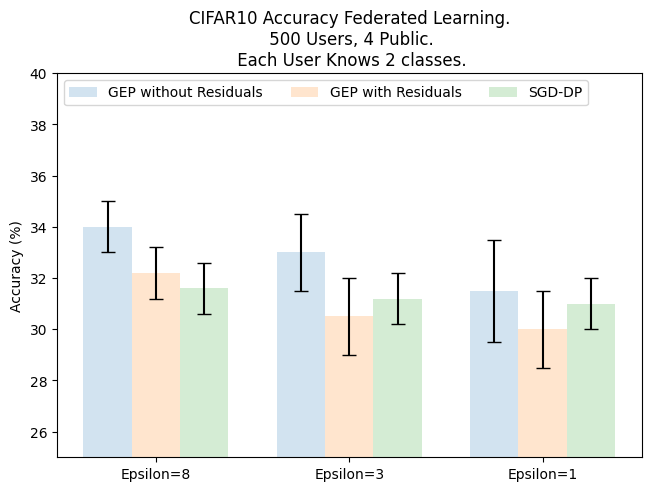
\includegraphics[height = 0.55\textwidth]{images/cifar10_dpsgd_vs_gep.png} \\
  From the initial results we see that if the privacy budget is $ \geq 3$, the advantage looks clear, but if it is low, the advantage is not so apparent. We hope to achieve better performance even for smaller privacy budget.

\printbibliography

\end{document}

